\documentclass[12pt]{article}
\usepackage[top=1in, bottom=1in, left=.75in, right=.75in]{geometry}
\usepackage{amsmath}
\usepackage{fancyhdr}
\usepackage{graphicx}
\usepackage{txfonts}
\usepackage{multicol}
\usepackage{adjustbox}
\usepackage[scaled=0.86]{helvet}
\renewcommand{\emph}[1]{\textsf{\textbf{#1}}}
\usepackage{anyfontsize}
% \usepackage{times}
% \usepackage[lf]{MinionPro}
\usepackage{tikz,pgfplots}
%\def\degC{{}^\circ{\rm C}}
\def\ra{\rightarrow}
\usetikzlibrary{calc}
\pgfplotsset{compat = newest}
\newcommand{\blank}[1]{\rule{#1}{0.75pt}}
\renewcommand{\d}{\displaystyle}
\newcommand{\ds}{\displaystyle}


\pgfplotsset{my style/.append style={axis x line=middle, axis y line=
middle, xlabel={$x$}, ylabel={$y$},axis equal}}

%yticklabels={,,} , xticklabels={,,}

% \setmainfont{Times}
% \def\sansfont{Lucida Grande Bold}
\parindent 0pt
\parskip 4pt
\pagestyle{fancy}
\fancyfoot[C]{\emph{\thepage}}
\fancyhead[L]{\ifnum \value{page} > 1\relax\emph{Math 251: Midterm 2}\fi}
\fancyhead[R]{\ifnum \value{page} > 1\relax\emph{November 11, 2021}\fi}
\headheight 15pt
\renewcommand{\headrulewidth}{0pt}
\renewcommand{\footrulewidth}{0pt}
\let\ds\displaystyle
\def\continued{{\emph {Continued....}}}
\def\continuing{{\emph {Problem \arabic{probcount} continued....}}\par\vskip 4pt}


\newcounter{probcount}
\newcounter{subprobcount}
\newcommand{\thesubproblem}{\emph{\alph{subprobcount}.}}
\def\problem#1{\setcounter{subprobcount}{0}%
\addtocounter{probcount}{1}{\emph{\arabic{probcount}.\hskip 1em(#1)}}\par}
\def\subproblem#1{\par\hangindent=1em\hangafter=0{%
\addtocounter{subprobcount}{1}\thesubproblem\emph{#1}\hskip 1em}}
\def\probskip{\vskip 10pt}
\def\medprobskip{\vskip 2in}
\def\subprobskip{\vskip 45pt}
\def\bigprobskip{\vskip 4in}

\begin{document}
{\emph{\fontsize{26}{28}\selectfont Math F251\hfill
{\fontsize{32}{36}\selectfont Midterm 2}
\hfill Fall 2021}}
\vskip 2cm
\strut\vtop{\halign{\emph#\hskip 0.5em\hfil&#\hbox to 2in{\hrulefill}\cr
\emph{\fontsize{18}{22}\selectfont Name:}&\cr
\noalign{\vskip 10pt}
%\emph{\fontsize{18}{22}\selectfont Student Id:}&\cr
%\noalign{\vskip 10pt}
%\emph{\fontsize{18}{22}\selectfont Calculator Model:}&\cr
}}
\hfill
\vtop{\halign{\emph{\fontsize{18}{22}\selectfont #}\hfil& \emph{\fontsize{18}{22}\selectfont\hskip 0.5ex $\square$ #}\hfil\cr
Section: & F01 (Jill Faudree)\cr
\noalign{\vskip 4pt}
         & F02 (James Gossell)\cr
\noalign{\vskip 4pt}
         & UX1 (James Gossell)\cr}}

\vfill
{\fontsize{18}{22}\selectfont\emph{Rules:}}

You have 60 minutes to complete the exam.  

Partial credit will be awarded, but you must show your work.

The exam is closed book and closed notes.

Calculators are not allowed. 


Place a box around your  \fbox{FINAL ANSWER} to each question where appropriate.

%If you need extra space, you can use the back sides of the pages.
%Please make it obvious  when you have done so.

Turn off anything that might go beep during the exam.

Good luck!
\vfill
\def\emptybox{\hbox to 2em{\vrule height 16pt depth 8pt width 0pt\hfil}}
\def\tline{\noalign{\hrule}}
\centerline{\vbox{\offinterlineskip
{
\bf\sf\fontsize{18pt}{22pt}\selectfont
\hrule
\halign{
\vrule#&\strut\quad\hfil#\hfil\quad&\vrule#&\quad\hfil#\hfil\quad
&\vrule#&\quad\hfil#\hfil\quad&\vrule#\cr
height 3pt&\omit&&\omit&&\omit&\cr
&Problem&&Possible&&Score&\cr\tline
height 3pt&\omit&&\omit&&\omit&\cr
&1&&12&&\emptybox&\cr\tline
&2&&6&&\emptybox&\cr\tline
&3&&12&&\emptybox&\cr\tline
&4&&20&&\emptybox&\cr\tline
&5&&12&&\emptybox&\cr\tline
&6&&8&&\emptybox&\cr\tline
&7&&10&&\emptybox&\cr\tline
&8&&10&&\emptybox&\cr\tline
&9&&10&&\emptybox&\cr\tline
%&Extra Credit&&3&&\emptybox&\cr\tline
&Total&&100&&\emptybox&\cr
}\hrule}}}

\newpage
\begin{enumerate}
\item (12 points) The volume of a cone is given by $V=\frac{1}{3}\pi r^2h$ where $r$ is the radius and $h$ is the height of the cone.
	\begin{enumerate}
	\item Assuming that the radius and the height are changing with time, $t$, find $\frac{dV}{dt}.$
	\vspace{2in}
	\item If the height of the cone decreases by $1$ inch per hour while the radius increases by $1$ inch per hour, find the rate of change of the volume of the cone at the moment when the radius is $10$ inches and the height is $5$ inches. Include units with your answer. Interpret your answer in the context of the problem
	\vfill
	\end{enumerate}  
	
%	\item Find the linearization of $f(x)=\sec x - \sin x$ centered at $a=0$.\\
%\vfill
\newpage
 \item (6 points) The radius of a spherical ball is measured to be $5$ inches with a possible error of $\pm 0.5$ inch. Use differentials to estimate the maximum possible error in the volume of the ball.\\
(Note: The volume of a sphere is given by $V=\frac{4}{3}\pi r^3$ where $r$ is the radius of the sphere.)\\
\vfill
\item (12 points)
\begin{multicols}{2}
	\begin{enumerate}
	\item Sketch a graph of a function $f(x)$ such that \\
	$f'(x)<0$ and \\
	$f''(x)>0$\\
	 for all real numbers $x.$\\
	 
	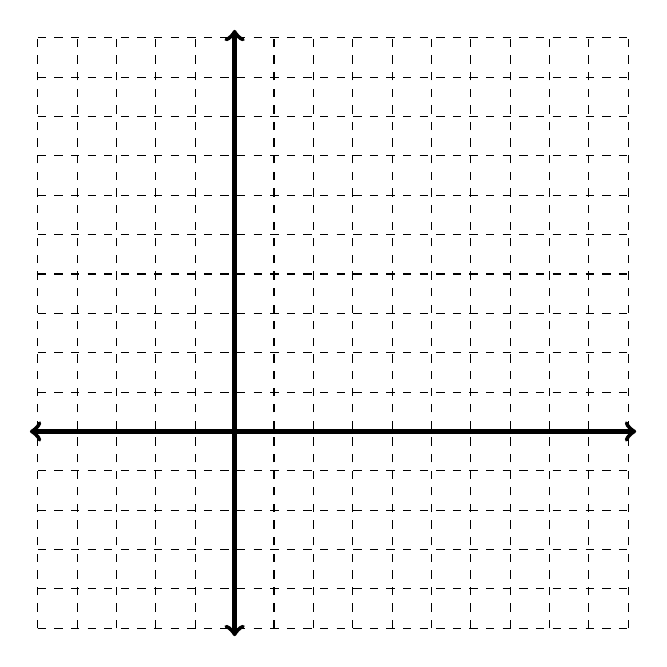
\begin{tikzpicture}[scale=.5]
	\draw[thin, dashed] (-5,-5) grid (10,10);
	\draw[<->, ultra thick] (-5.2,0) -- (10.2,0);
	\draw[<->,ultra thick] (0,-5.2) -- (0, 10.2);
\end{tikzpicture}
	
	\item Sketch a graph of a function $f(x)$ such that\\
	 $f'(0)=0$, \\
	 $f''(x)> 0 $ when $x<0$, and  \\
	 $f''(x)<0$ when $x >0$.
	
	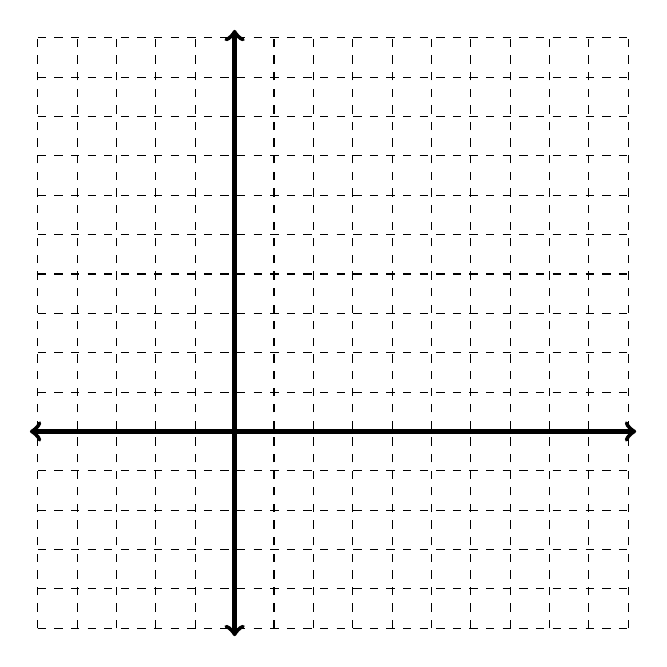
\begin{tikzpicture}[scale=.5]
	\draw[thin, dashed] (-5,-5) grid (10,10);
	\draw[<->, ultra thick] (-5.2,0) -- (10.2,0);
	\draw[<->,ultra thick] (0,-5.2) -- (0, 10.2);
\end{tikzpicture}
	\end{enumerate}
	\end{multicols}
\newpage
%%Cirt pts intervals of increase/decrease
\item (20 points) Use the information below to answer questions about the function $f(x).$ Make sure you answer the question!  \\
$$f(x)=\frac{2x^2-1}{x^2+3}, \hspace{.2in} f'(x)=\frac{14x}{(x^2+3)^2},
\hspace{.2in} f''(x)=\frac{-42(x^2-1)}{(x^2+3)^3}.$$

\begin{enumerate}
\item  Determine the intervals on which $f(x)$ is increasing/decreasing.
\vfill
\item Find the local maximum/minimum values of $f(x)$. If something doesn't exist, you must explicitly state this and justify your answer.
\vfill
%\vskip1.35in
\item Find the intervals on which $f(x)$ is concave up and concave down.
\vfill 
\item Find any inflection points of $f(x).$ If there aren't any, you must explicitly state this and justify your answer.
\vfill
\item Find any horizontal asymptotes of $f(x)$ or state that none exist. Justify your answer.
\vfill
\end{enumerate}
\newpage
%optimixation
\item (12 points) Find the pair of numbers $x$ and $y$ on the line $3x+y=15$ such that the product $(x+2)(y-3)$ is as large as possible. 
	\begin{enumerate}
	\item Explicitly state the quantity you want to maximize or minimize.
	\item Identify the domain of your function.
	\item Identify your answer. (Note: Your answer may not be an integer.)
	\item Justify that your answer is correct. That is, use Calculus to show that your answer indeed does represent a maximum or minimum.
	\end{enumerate}
\newpage

\item  (8 points) Evaluate the following limit using L'Hopital's Rule. Before each application of L'Hopital's Rule, you must indicate the form of the limit ($0/0$ or $\infty/\infty$).\\
\vspace{.2in}
$$\lim_{x \rightarrow 0}\frac{\ln(\sin x + \cos x)}{x}$$

\vfill

\item (10 points)  Evaluate the following indefinite integrals:

\begin{enumerate}
\item $\ds \int x(x-1)\:dx$
\vfill
\item $\ds \int \left(\sec^2x - e^x + \frac{1}{\sqrt{1-x^2}}\right)\:dx$
\vfill
\end{enumerate}

\newpage
\item (10 points) A drone is released into the air from an initial height of $5$ feet off the ground. Its upward velocity at $t$ seconds is $v(t) = 3t^2 - 3$ feet per second. How high will the drone be after $2$ seconds?
%%% use derivatives get shape of graph
\vfill

%\item  Given $f(x) = \frac{10}{1+x}$, approximate the area (shaded in gray) bounded between the graph of $f(x)$, the $x$-axis and the lines $x = 1$ and $x= 10$ using $L_3$:  three rectangles determined by left-hand endpoints.  {\bf Draw and shade in the rectangles you are using on the graph.} Show your computation clearly. You do not need to simplify your answer. Indicate whether your estimate is an over-estimate or an under estimate.
%
%\begin{tikzpicture}[xscale = 0.7,yscale=0.5]
%\draw[draw=gray!20!white,fill=gray!20!white] 
%    plot[smooth,samples=100,domain=1:10] ({\x,10/(1+\x)}) -- 
%    (10,0) -- (1,0) -- (1,5);
% \draw[ultra thick,<-> ] plot[smooth, domain=-.25:11]({\x,10/(1+\x)});
%\foreach \i in {1,3,5,7,9}{
%	\draw (\i, 1/4)--(\i,0) node[below] {$\i$};}
%\foreach \i in {2,4,6,8,10}{
%	\draw (\i, 1/4)--(\i,0){};}
%
%\draw[<->] (-1,0) -- (12,0);
%\draw[<->] (0,-1) -- (0, 12);
%%\draw (.1, 1/2)-- (-.1, 1/2) node[left]{{\small $\nicefrac{1}{2}$}} ;
%%\draw (.1, 1/4)-- (-.1, 1/4) node[left]{{\small $\nicefrac{1}{4}$}} ;
%%\draw (.1, 3/4)-- (-.1, 3/4) node[left]{{\small $\nicefrac{3}{4}$}} ;
%%\draw (.1, 1)-- (-.1, 1) node[left]{{\small 1}} ;
%
%\end{tikzpicture}

%\newpage
\item (10 points) Using the graph of $f(x)$ shown (below) and  geometry, calculate exactly each of the following quantities. Show your work to receive partial credit.


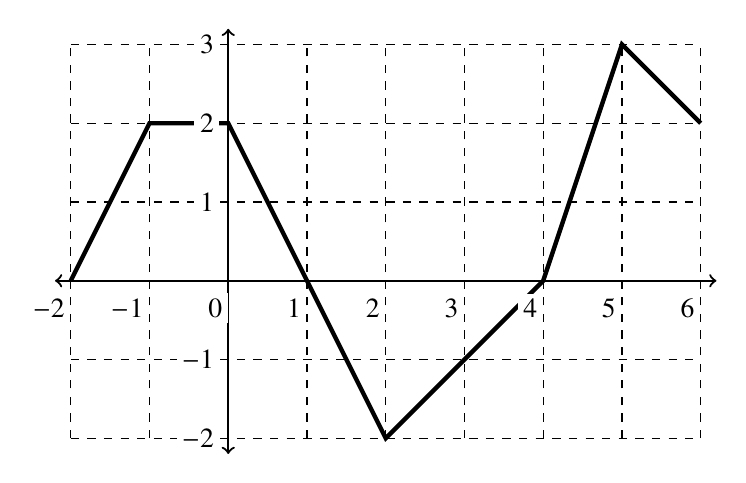
\begin{tikzpicture}[scale=1]
\draw[thin, dashed] (-2,-2) grid (6,3);
\draw[<->, thick] (-2.2,0) -- (6.2,0);
\draw[<->, thick] (0,-2.2) -- (0, 3.2);
\draw[ultra thick] (-2,0) -- (-1,2) -- (0,2) -- (2,-2) -- (4,0)  --(5,3)-- (6,2);

\foreach \i in {-2, -1,1,2, 3}{\draw (0,\i) node[left=3 pt,fill=white, inner sep=2pt] {$\i$};}
\foreach \i in {-2, -1,0,1,2, 3,4,5,6}{\draw (\i,0) node[below=10pt, left= .01 pt, fill=white, inner sep=2pt] {$\i$};}

\end{tikzpicture}

\begin{enumerate}
\item $\d \int_{-2}^{4} f(x) \ dx =$ 
\vspace{.5in}

\item $\d \int_{-2}^1 (2 f(x)+5) \ dx$ =
\vspace{.5in}

\end{enumerate}


\end{enumerate}
\end{document}
